\documentclass[10pt]{article}
    \usepackage{listings}
    \usepackage{xcolor}
    \usepackage{graphicx}
    \usepackage{pythonhighlight}
    \usepackage{amsmath}
    \usepackage[left = 2cm,right = 2cm,top = 3 cm,bottom = 3cm]{geometry}
\lstset{columns = fixed,
 numbers = left,
 frame = none,
 backgroundcolor = \color[RGB]{240,244,245},
 keywordstyle = \color[RGB]{0,0,255},
 numberstyle = \footnotesize\color{darkgray},
 commentstyle = \it\color[RGB]{255,96,96},
 stringstyle = \rmfamily\slshape\color[RGB]{255,0,255},
 showstringspaces = false,
 language=C++,
 }
 \begin{document}
     \title{Study Report}
     \author{Shuo Xu}
     \maketitle
     \begin{abstract}
         This report is mainly about the derivation process of the formulas backpropagation and calculation method of matrix form.
     \end{abstract}

     \begin{center}

         \section*{Derication pross}

         
         \begin{figure}[h]
            \centering
            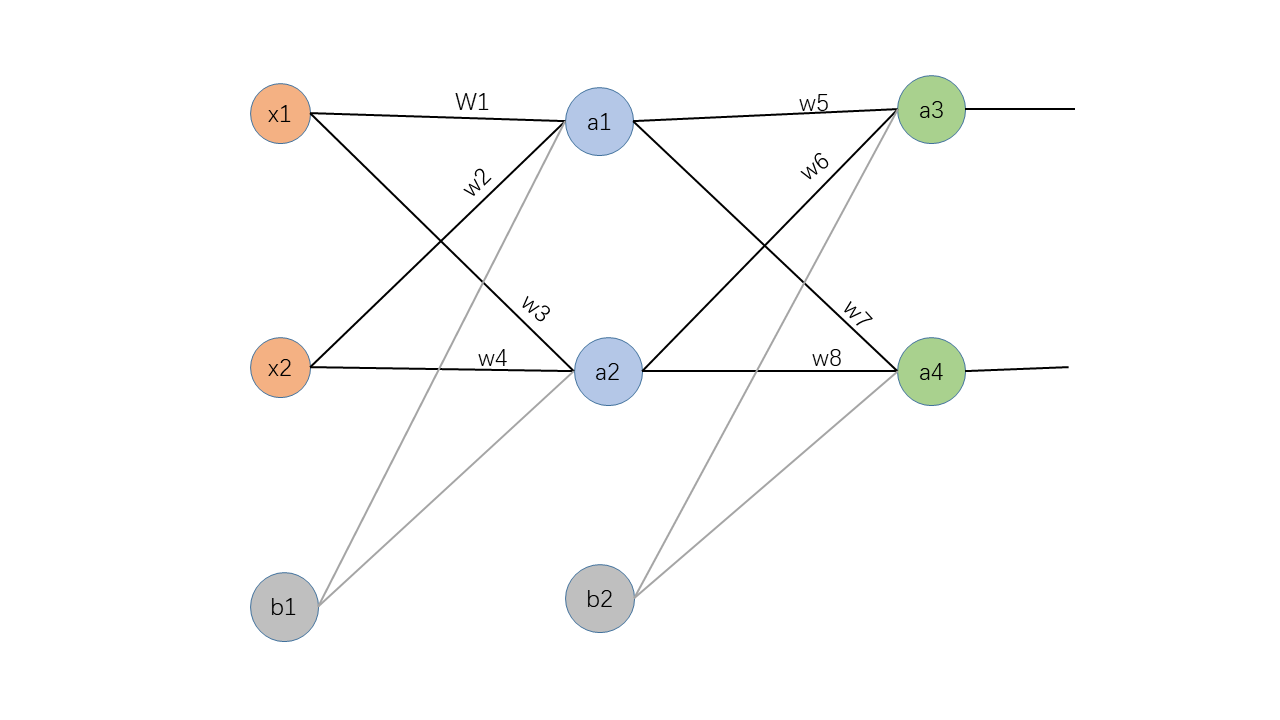
\includegraphics[scale=0.45]{bp2.png}
            \caption{neural network}
            \label{fig:label}
        \end{figure}
         \begin{flushleft}
            My derivation is about the picture above, and the following are the formulas I will use.
                $$Z^{[l]} = W^{[l]}A^{[l-1]}+b^{[l]}\eqno(1)$$
                $$A^{[l]} = f(Z^{[l]}) = \frac{1}{1+e^{-Z^{[l]}}}\eqno(2)$$
                $$L = \frac{1}{2}\sum(Y-A)^{2}  \eqno(3)$$  %均方误差
                $$sigmoid:dZ^{[l]} = f'(Z^{[l]}) = f(Z^{[l]})(1 - f(Z^{[l]})) = A^{[l]}(1-A^{[l]}) .\eqno(4)$$
            The upper case letters in the formula are all matrix forms, I will first complete the computation one by one, and then simplify the expression in matrix form.
         \end{flushleft}
             
     \end{center}
     \subsection*{Forward propagation}
     \begin{flushleft}
        $z_{1} = w_{1}x_{1} + w_{2}x_{2} + b_1$ \quad $z_{2} = w_{3}x_{1} + w_{4}x_{2} + b_1$ \quad $a_{1} = \frac{1}{1+e^{-z_{1}}}$ \quad $a_{2} = \frac{1}{1+e^{-z_{2}}}$\vspace{1ex}

        $z_{3} = w_{5}a_{1} + w_{6}a_{2} + b_2$ \quad $z_{4} = w_{7}a_{1} + w_{8}a_{2} + b_2$ \quad $a_{3} = \frac{1}{1+e^{-z_{3}}}$ \quad $a_{4} = \frac{1}{1+e^{-z_{4}}}$\vspace{1ex}

        $L = L_1 + L_2 = \frac{1}{2}(y_1 - a_3)^2 +  \frac{1}{2}(y_2 - a_4)^2$ \vspace{3ex}

        If we use the matrix form to simplify the upper expression:\vspace{3ex}
        
        \begin{center}
        $A_0 = X = \begin{bmatrix}
            x_1 \\
            x_2
        \end{bmatrix}$ \quad
        $Z_1 = \begin{bmatrix}
            z_1 \\
            z_2
        \end{bmatrix}$ \quad
        $A_1 = \begin{bmatrix}
            a_1 \\
            a_2
        \end{bmatrix}$ \quad
        $Z_2 = \begin{bmatrix}
            z_3 \\
            z_4
        \end{bmatrix}$ \quad
        $A_2 = \begin{bmatrix}
            a_3 \\
            a_4
        \end{bmatrix}$ \vspace{3ex}
        \end{center}

        We have known the unmpy package in Python, according to its broadcast, b does not need to be processed. If we want to use matrix to simplify, the W we need are: \vspace{3ex}

        \begin{center}
        $W_1 = \begin{bmatrix}
            w_1  & w_2\\
            w_3  & w_4
        \end{bmatrix}$ \quad
        $W_2 = \begin{bmatrix}
            w_5 & w_6\\
            w_7 & w_8
        \end{bmatrix}$ \vspace{3ex}
        \end{center}
        In this case, we can use the formula 1 and 2, and if we use many examples to make the matrix X, these formulas are also effective. In order to facilitate my expression, I do not list this situation here.
     \end{flushleft} 

    \subsection*{Backward propagation}
    \begin{flushleft}
        Because the backward propagation is a little complicated, I will only talk about the top path. According to the chain rule we have:\vspace{3ex}

        $da_3 = \frac{\partial L}{\partial a_3} = \frac{\partial L_1}{\partial a_3} = a_3 - y_1$ \qquad    
        $dz_3 = \frac{\partial L}{\partial z_3} = da_3\frac{\partial a_3}{\partial z_3} = da_3\times a_3(1-a_3)$ \qquad 
        $dw_5 = \frac{\partial L}{\partial w_5} = dz_3\frac{\partial z_3}{\partial w_5} = dz_3\times a_1$ \vspace{2ex}

        In the figure 1 we can see $w_5$ and $w_7$ are connected to $a_1$, if we want to calculate $da_1$, we need use two routes and that's the same to $a_2$, $b_2$ and $b_1$. Fortunately we don't need to calculate $dx$, and if we use the matrix, all the thing will be simple.\vspace{3ex}
        
        $da_1= \frac{\partial L}{\partial a_1} = \frac{\partial L1}{\partial a_1} + \frac{\partial L2}{\partial a_1} = dz_3\frac{\partial z_3}{\partial a_1} + dz_4\frac{\partial z_4}{\partial a_1} = dz_3 \times w_5 + dz_4 \times w_7$ \vspace{1ex}
        
        $dw_1 = \frac{\partial L}{\partial w_1} = da_1\frac{\partial a_1}{\partial w_1} = da_1\times a_1(1-a_1)$ \vspace{1ex}
        
        $db_2 = \frac{\partial L}{\partial b_2} = \frac{1}{2}(dz_3 \frac{\partial z_3}{\partial b_2} + dz_4 \frac{\partial z_4}{\partial b_2}) =\frac{1}{2}(dz_3+dz_4)$ \qquad ($b$ only have one example.)\vspace{3ex}

        Use matrix to simplify:
        \begin{center}
            $dZ_1 = \begin{bmatrix}
                db_1 \\
                db_2
            \end{bmatrix}$ \quad
            $dA_1 = \begin{bmatrix}
                da_1 \\
                da_2
            \end{bmatrix}$ \quad
            $dZ_2 = \begin{bmatrix}
                db_3 \\
                db_4
            \end{bmatrix}$ \quad
            $dA_2 = \begin{bmatrix}
                da_3 \\
                da_4
            \end{bmatrix}$ \vspace{3ex}
        \end{center}
        
        We can calculate the $dZ$ and $dA$ of the output layer according to different function. But the way to calculate $dW$ , $dB$ and another especial one, $dA^{[l-1]}$, is same in every neural network. According to the formula 1 we will have:

        $$ dW^{[l]} = \frac{1}{m} dZ^{[l]}A^{[l-1]T} \eqno(5)$$
        $$ db^{[l]} = \frac{1}{m} \sum_{i=1}^{m}dZ^{[l](i)} \eqno(6)$$
        $$ dA^{[l-1]} = W^{[l]T}dZ^{[l]} \eqno(7)$$
        Here I will give some instructions. In the example that I give, we can easily find the way to calculate $dW$ as formula 5, but if we want to calculate many datas at the same time, we shuld add the $\frac{1}{m}$.
    \end{flushleft}

    \subsection*{Update}
    \begin{flushleft}
        We use $\alpha$ as the learning rate, so now we can upadte the parameters, using gradient descent.\vspace{3ex}
        \begin{center}
            $   w_1 = w_1 - \alpha dw_1$ \qquad
            $   b_1 = b_1 - \alpha db_1$ \vspace{3ex}
        \end{center}
        Use matrix to simplify:

        $$ W^{[l]} = W^{[l]} - \alpha \text{ } dW^{[l]} $$
        $$ b^{[l]} = b^{[l]} - \alpha \text{ } db^{[l]} $$
    \end{flushleft}

    \begin{flushleft}
      
        

    \end{flushleft}
    \begin{center}
        \section*{Leetcode}
    \end{center}
        \subsection*{Description}
        Given a string of numbers and operators, return all possible results from computing all the different possible ways to group numbers and operators. The valid operators are +, - and *.

        Example 1: \qquad Input: "2-1-1" \qquad Output: [0, 2]

        Explanation: \qquad ((2-1)-1) = 0 \qquad (2-(1-1)) = 2

        Example 2: \qquad Input: "2*3-4*5" \qquad Output: [-34, -14, -10, -10, 10]

        Explanation: \qquad (2*(3-(4*5))) = -34 \qquad ((2*3)-(4*5)) = -14 \qquad ((2*(3-4))*5) = -10 \qquad (2*((3-4)*5)) = -10 \qquad (((2*3)-4)*5) = 10

        \subsection*{Solution}
        This problem dosen't require us to make sure the return vector don't contain repeating elements, so it's easy to solve it. Traverse the string, if we find an operator, divide the string into two parts in this position and use the function itself to get two vectors. Then use the operator that we found to calculate all combinations of two vectors, and add every result to the final vector.

        \newpage

        \subsection*{Code}
        \begin{lstlisting}
class Solution {
public:
    vector<int> diffWaysToCompute(string input) {
        vector<int> res;
        for(int i = 0; i < input.size(); i++){
            if(input[i] < '0'){
                vector<int> left = diffWaysToCompute(input.substr(0,i));
                vector<int> right = diffWaysToCompute(input.substr(i + 1));
                for(int j = 0; j < left.size(); j++)
                    for(int k = 0; k < right.size(); k++){
                        if(input[i] == '+')
                            res.push_back(left[j] + right[k]);
                        else if(input[i] == '-')
                            res.push_back(left[j] - right[k]);
                        else
                            res.push_back(left[j] * right[k]);
                    }
            }
        }
        if(res.empty())
            res.push_back(atoi(input.c_str()));  
        return res;
    }
};
        \end{lstlisting}


        \section*{Others}
        I want to know where we shuld use linux. And maybe the MLP still have something wrong. I was surprised by the curve drawn by the program. I don't understand why the part of the beginning of the curve is horizontal. 5000 epoches is enough for my program.
        

\end{document}

